% \documentclass[fleqn,10pt]{wlscirep}
% \usepackage[utf8]{inputenc}
% \usepackage[T1]{fontenc}
% \usepackage{float}
% \usepackage{xcolor}
% \usepackage{enumitem,amssymb}
% \usepackage{subcaption}
% \newlist{checklist}{itemize}{2}
% \setlist[checklist]{label=$\square$}
% \usepackage{longtable}
% \usepackage{soul}
% \usepackage{longtable}
% \newcommand{\notateThiago}[1]{\textcolor{blue}{\textbf{[#1]}}}
% \newcommand{\notateJay}[1]{\textcolor{red}{\textbf{[#1]}}}
% \newcommand{\doiprefix}{}
% \counterwithin{figure}{section}


% \title{In-flight positional and energy use data set of a DJI
% Matrice 100 quadcopter for small package delivery
% : Supplementary information}
% \begin{document}
% \author{}
% \maketitle

\section{检查清单}
\subsection{飞行前}
\label{apen1:pre}

\begin{checklist}
    \item 检查飞行器
    \begin{checklist}
        \item 目视检查无人机系统各部件的状态
        \item 检查机体结构，包括起落架、所有飞行控制面及其连接机构
        \item 检查注册标识是否展示正确且清晰可读
        \item 检查可动控制面及其机体连接点
        \item 检查舵机及其连接点
        \item 检查推进系统，包括动力装置、螺旋桨、旋翼、涵道风扇等
    \end{checklist}
    \item 确认所有系统（如飞行器、控制单元）都具有满足本次任务的足够电量，并正常工作
    \item 检查航电系统，包括控制链路收发器、通信/导航设备及天线
    \item 检查 UAS 罗盘，并在必要时于飞行前重新校准
    % \item Inspect the control link transceiver, communication/navigation data link transceiver, and antenna(s)
    \item 如使用显示面板，检查其是否工作正常
    \item 检查地面保障设备（包括起飞与着陆系统）是否运行正常
    % \item Check that control link correct functionality is established between the aircraft and the control station
    % \item Check for correct movement of control surfaces using the control station
    \item 检查机载导航与通信数据链路
    \item 检查飞行终止系统和人工接管开关
    % \item Check fuel for correct type and quantity
    \item 检查飞行器和地面控制站的电池电量
    \item 检查载荷是否安装牢固
    \item 确认与 UAS 通信正常，并确认 UAS 已从至少 4 颗卫星获得 GPS 定位
    \item 执行一次螺旋桨上锁和解锁，以检查是否存在不平衡或异常运转
    % \item Verify all controller operation for heading and altitude
    \item 如飞行路径踏勘提出要求，确认所有可能干扰 UAS 的障碍物
    \item 在可控低高度下进行人工飞行测试，验证是否存在干扰，并重新检查所有控制量与稳定性
\end{checklist}

\subsection{飞行后}
\label{apen1:post}
% \subsection*{Pre-landing}
% \begin{checklist}
%     \item Ensure that the LZ (landing zone) is clear, otherwise abort and proceed to alternative LZ
%     \item Pilot calls "Landing"
%     \item Initiate auto land either using the app or programming code
% \end{checklist}

% \subsection*{Post-landing}
\begin{checklist}
    \item 等待所有电机和旋翼完全停止
    \item 确认传感器记录已经停止
    \item 断开电池
    \item 检查机体是否存在飞行中损伤
    \item 检查线缆是否固定牢靠
    \item 检查所有连接器是否完全连接
    \item 检查电机是否安装牢固
    \item 检查螺旋桨是否固定可靠
    \item 检查螺旋桨是否能在无阻碍条件下自由转动（例如不会碰到安装错误的防护罩边缘），或确认其已拆除
    \item 确认所有传感器无遮挡且未受损
\end{checklist}

\section{风速计幅值偏差与自运动修正}
\label{chap:bias}

消除风测量中幅值偏差和自运动影响的一种方法，是结合惯性速度数据以及 Brushi 等人 \cite{bruschi2016wind} 在风洞中使用带超声风传感器的四旋翼所采集的数据。由于他们的实验布置与我们的配置相近，我们使用其风洞实验结果 \cite{bruschi2016wind} 来构建测量风速与真实风速之间的多项式映射。由于原始数据在低数值区间的数据点不足，我们又加入了本实验装置得到的结果进行补充。数据点及其拟合曲线见图 \ref{fig:anemo_usage}。为了获得低数值区间的数据，我们让 UAV 在近零风条件下以悬停和恒定地速模式持续飞行较长时间。幅值修正多项式和自运动修正方法如式 \ref{eq:corr} 所示。
\begin{equation}
    \begin{split}
% V &= \sqrt{V_N^2 + V_E^2}\\
w_m^{[actual]} &= -0.002(w_m^{[raw]})^4 + 0.052(w_m^{[raw]})^3-0.421(w_m^{[raw]})^2 + 1.917w_m^{[raw]} - 2.7\\
w_N &= (w_m^{[actual]})\cos(w_{\theta}^{[raw]}) - V_N\\
w_E &= (w_m^{[actual]})\sin(w_{\theta}^{[raw]}) - V_E\\
w_m^{[corrected]} &= \sqrt{w_N^2 + w_E^2}\\
w_{\theta}^{[corrected]} &= \arctan(w_E,w_N)\\
\end{split}
\label{eq:corr}
\end{equation}
其中，$V_N$ 和 $V_E$ 分别表示 UAV 在北向和东向的惯性速度，$w_N$ 和 $w_E$ 分别表示修正后的北向和东向风分量。 
\begin{figure} [H]
    \centering
    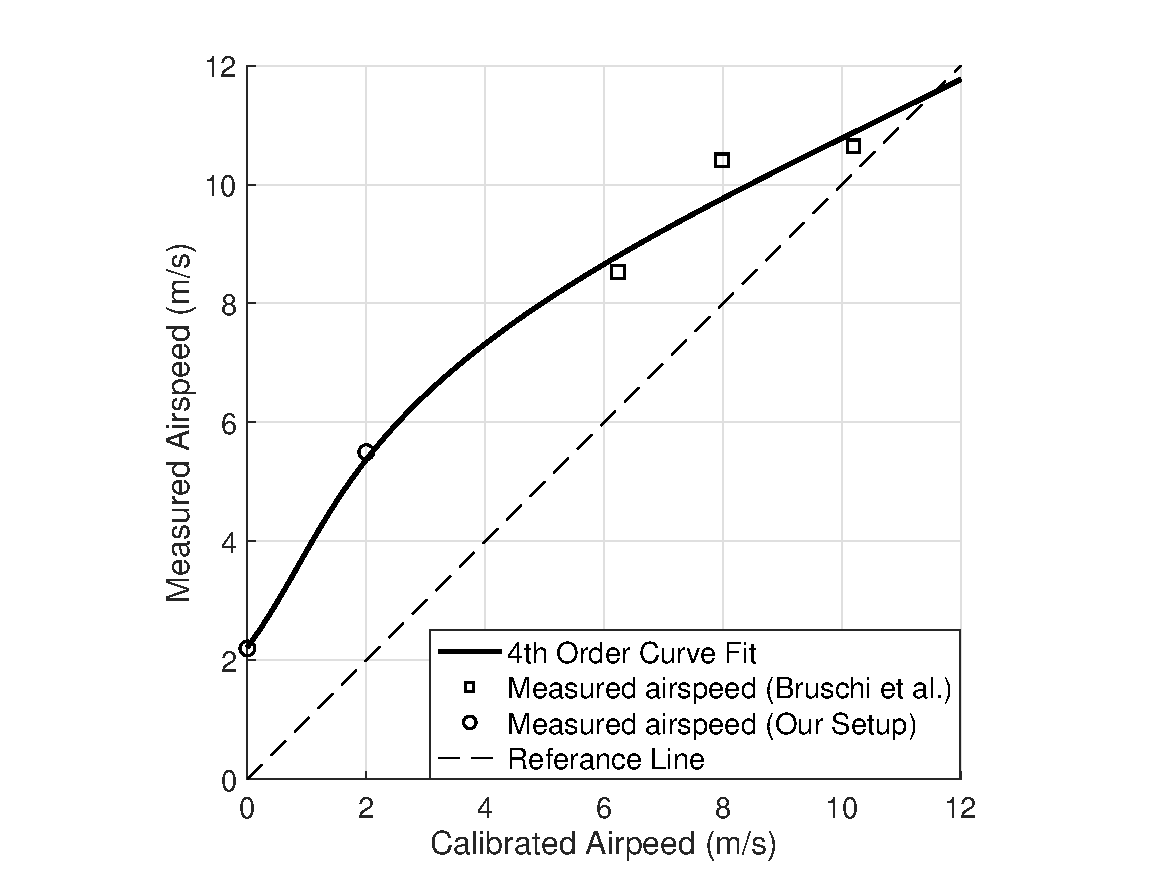
\includegraphics[width=0.45\textwidth]{figures/figure11.pdf}
    \caption{风速计修正结果}
    \label{fig:anemo_usage}
\end{figure}

数据集保留的是原始测量值，并未使用上述方法进行修正，因为本研究的重点并不在于获得高精度风场估计。利用无人机进行风估计本身仍是一个持续发展的研究方向\cite{Patrikar-2020-125335}，原因在于旋翼会引入复杂的气流扰动，从而影响风速计的测量。因此，我们保留原始数据形式，以便在需要时应用当前或未来各种风修正方法。

% \end{document}
